\documentclass{beamer}
\usepackage[utf8]{inputenc}
\usetheme{Copenhagen}
\usecolortheme{seahorse}

\title{Implementacija osnovnih git komandi}
\author{Adrian Bralic Toth \and Anton Frlan}
\institute{Tehnički Fakultet Rijeka}
\date{2018}

\begin{document}

\frame{\titlepage}

\begin{frame}{git init}

\begin{itemize}
	\setlength\itemsep{2em}
	\item Git init stvori .git datoteku te ostale u njoj napravi još neke datoteke potrebne za rad git-a.
	\begin{figure}
\centering
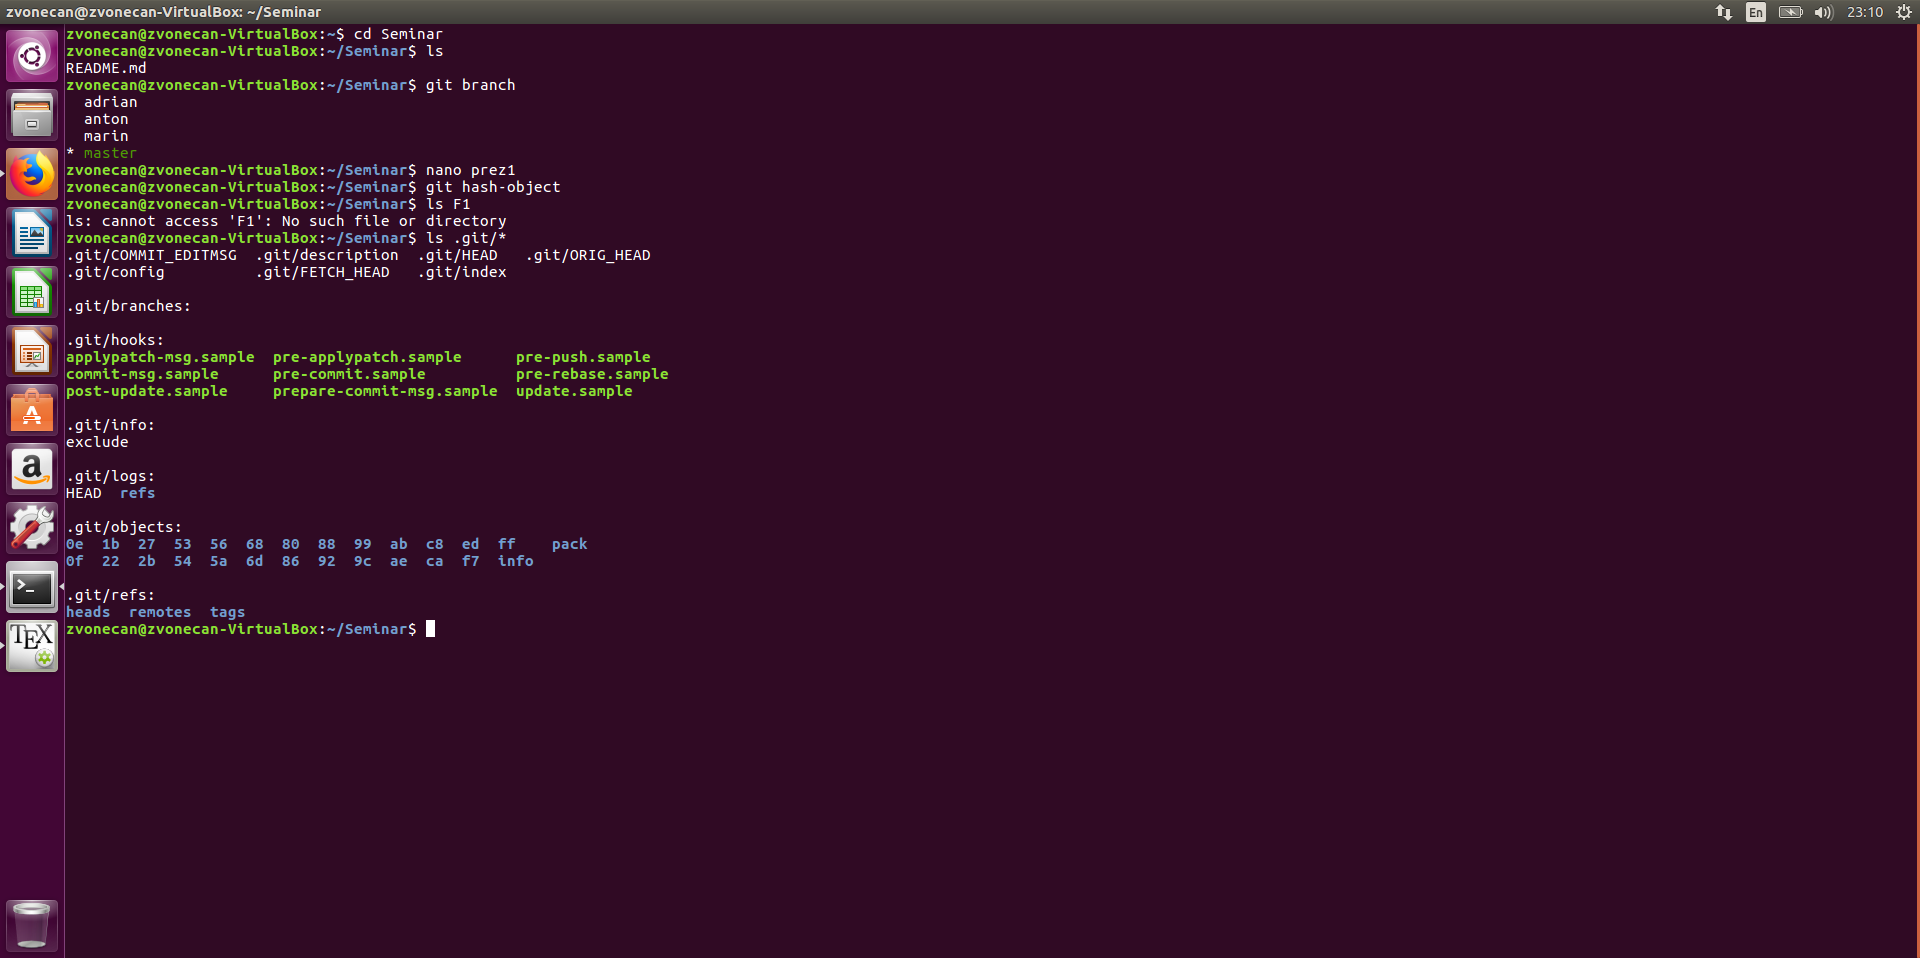
\includegraphics[width=0.9\textwidth]{./slike/git_datoteka.png}
\end{figure}
\end{itemize}

\end{frame}

\begin{frame}{Clone i config}

\begin{itemize}
	\item Clone funkcionira vrlo slično git initu, ali kopira već gotov repozitrorij s udaljene lokacije.
\end{itemize}
	\begin{figure}
		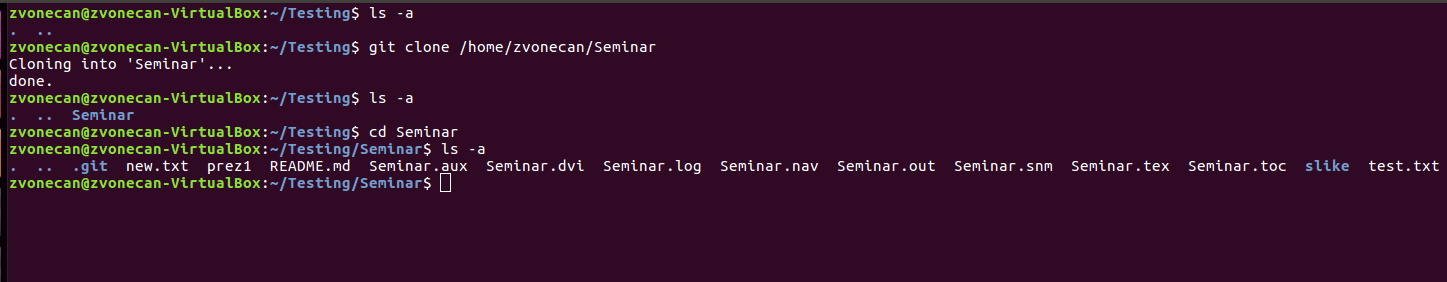
\includegraphics[width=0.9\textwidth]{./slike/b.png}
	\end{figure}
\begin{itemize}
	\item Pomoću naredbe config postavljamo username i email od korisnika
\end{itemize}

\end{frame}



\begin{frame}{git commit}

\begin{itemize}
	\setlength\itemsep{2.5em}
	\item Git commit git izvršava tako da datoteku spremi pod ključ zvan SHA-1.
	\item SHA-1 je kombinacija od 40 malih slova ili brojeva koja služi kao pointer na spremljenu datoteku.
	\item Pomoću komande git hash-object možemo spremi neki file u git te dodavanjem -w nam git vraća SHA-1 od tog filea.
	\item Pomoću git hash-object spremamo neki file pod SHA-1 kao blob i možemo mu pristupiti samo pomoću SHA-1 ključa.
\end{itemize}

\end{frame}

\begin{frame}{git commit}
\begin{figure}
\centering
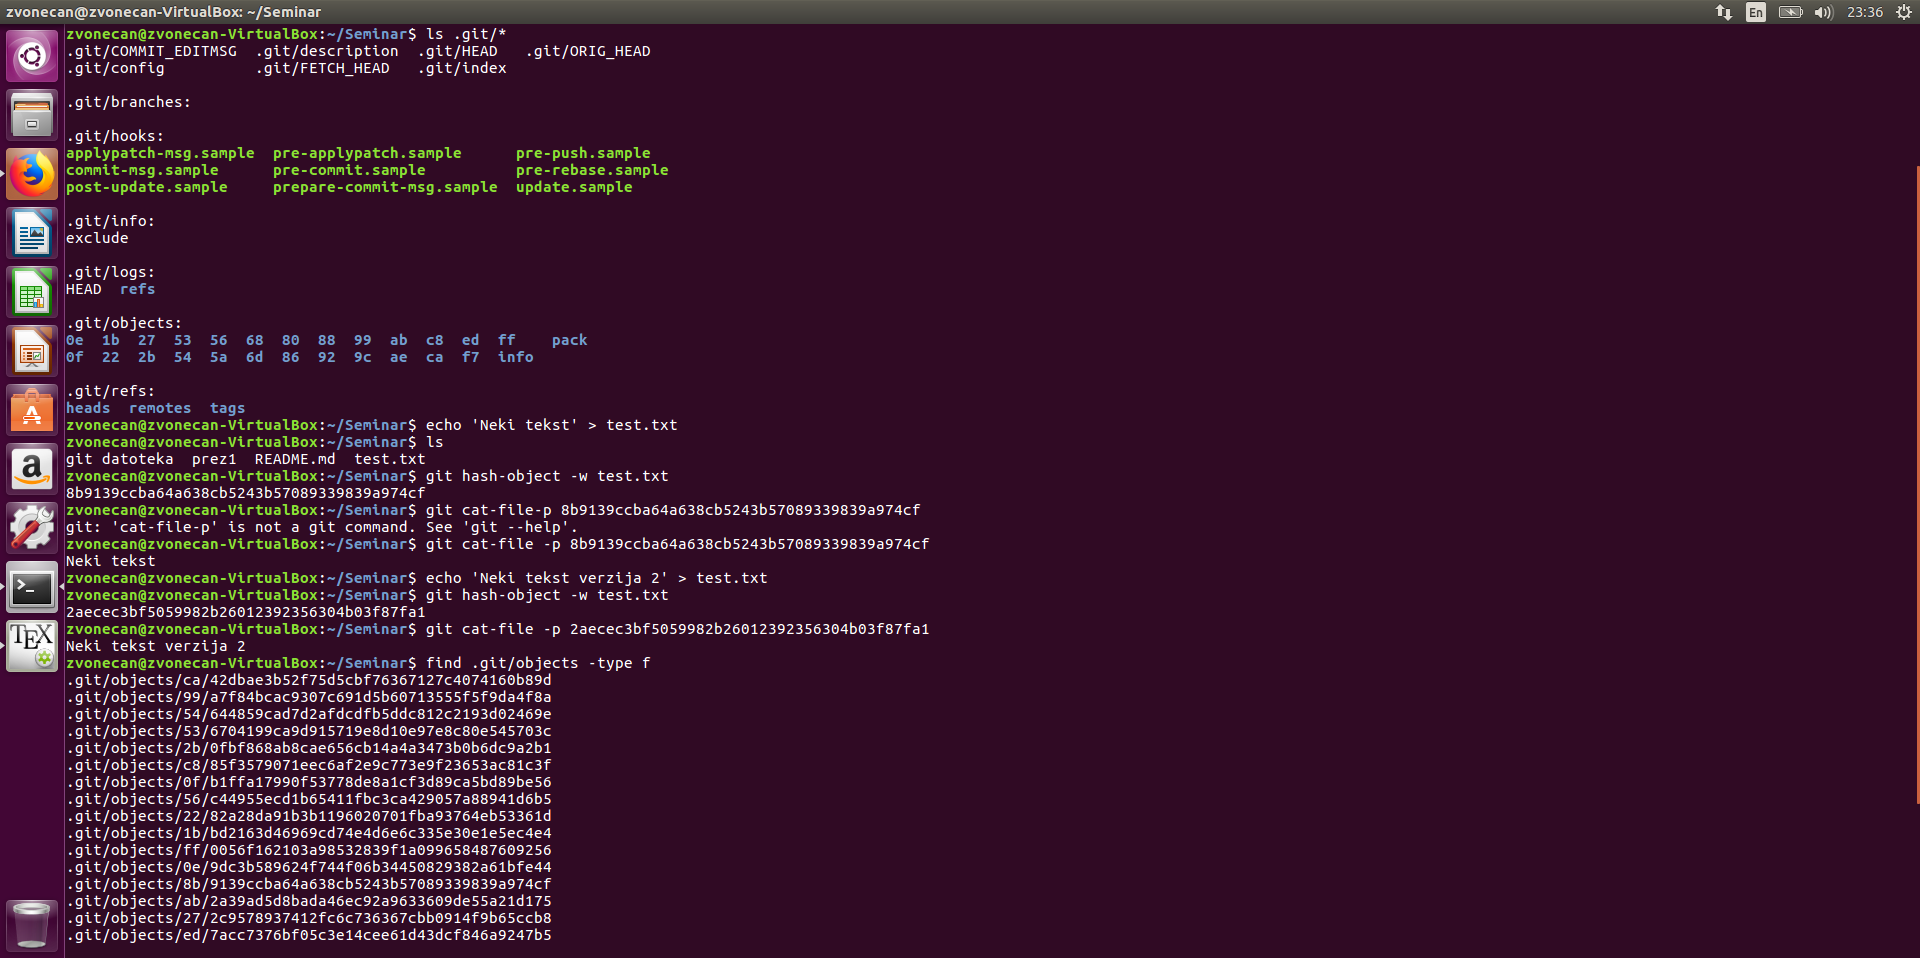
\includegraphics[width=0.9\textwidth]{./slike/druga_slika.png}
\end{figure}

\end{frame}

\begin{frame}{git commit}

\begin{itemize}
	\item Git rješava taj problem pomoću stabala.
	\item Blob je neki podatak ili tekst dok je stablo vise blobova i barem jedno stablo od kojih jedno stablo ima SHA-1 te datoteke ili stabla koji ga sadrži.
	\begin{figure}
		\centering
	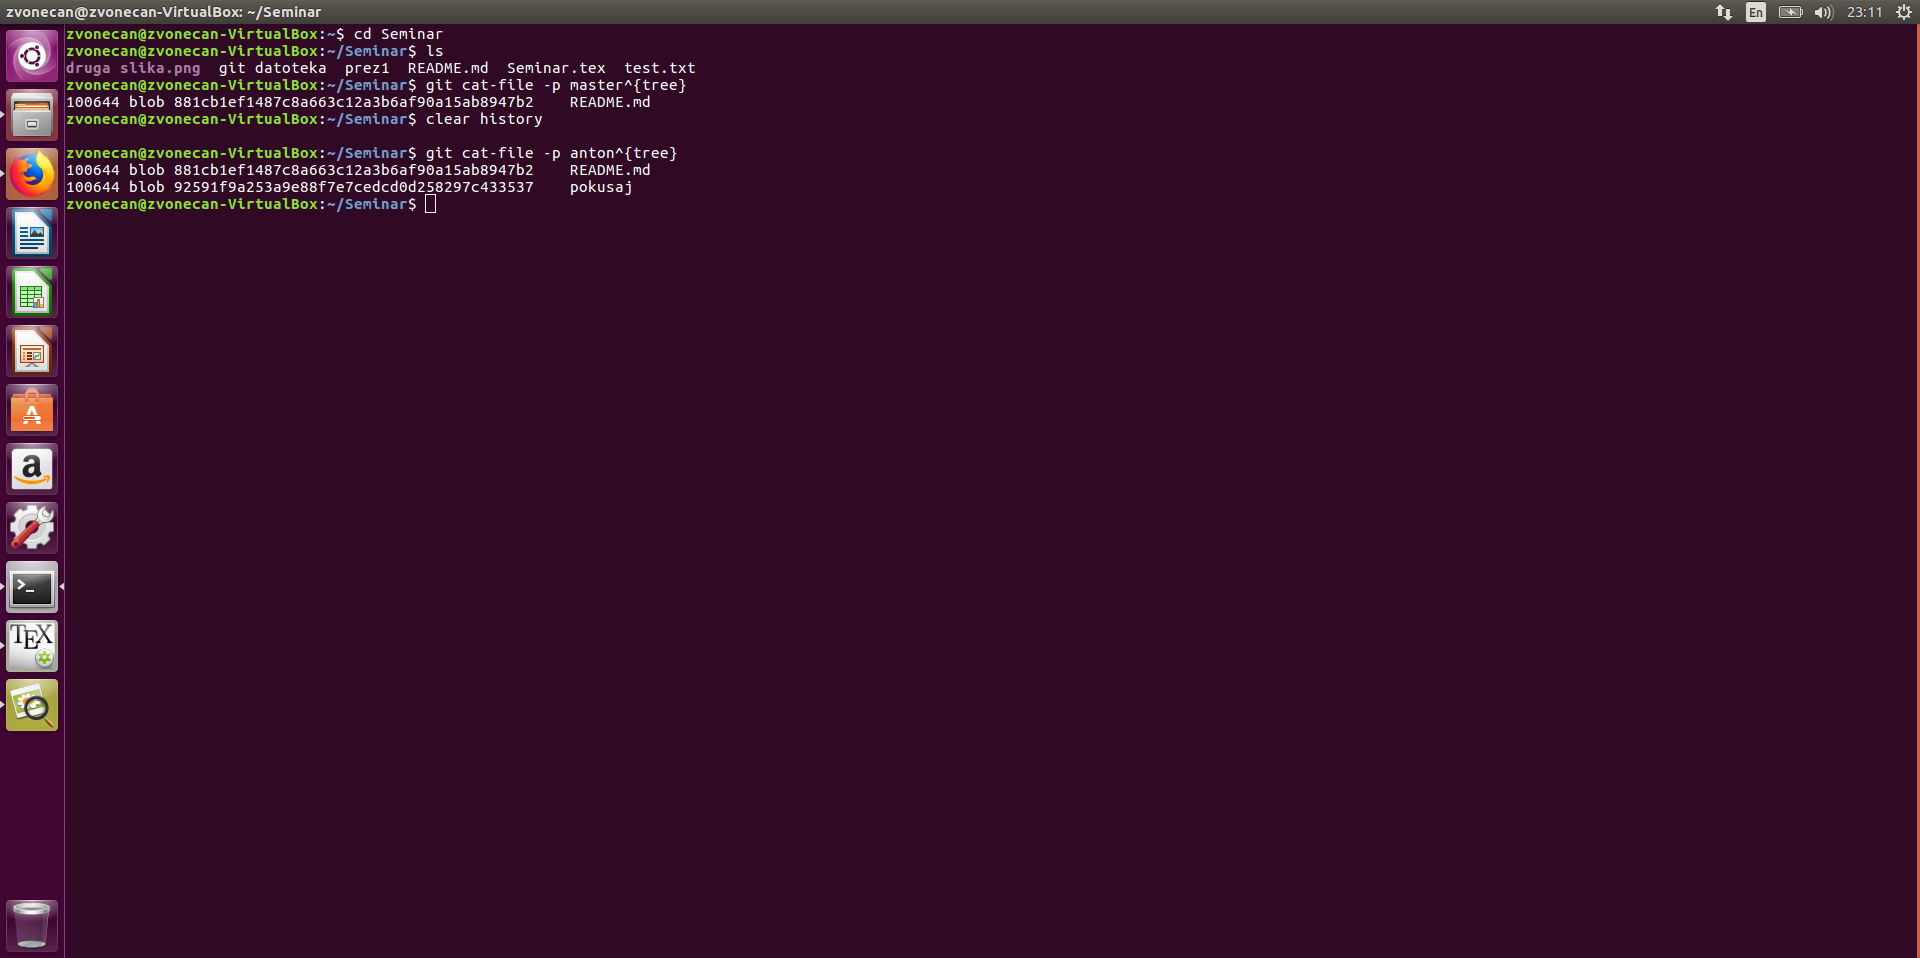
\includegraphics[width=0.5\textwidth]{./slike/treca_slika.png}
	\end{figure}
	\item Kada git commita file on obično uzme sto je na stage-u i spremi u jedno stablo ili kombinaciju stabala koji su svi spremljeni pod jedno stablo.
\end{itemize}
\end{frame}

\begin{frame}{git stage}

\begin{itemize}
	\item File u gitu stageamo tako da ga dodamo u pod datoteku index unutar .git datoteke.
	\item File dodajemo u index pomoću git update-index --add.
	\begin{figure}
		\centering
	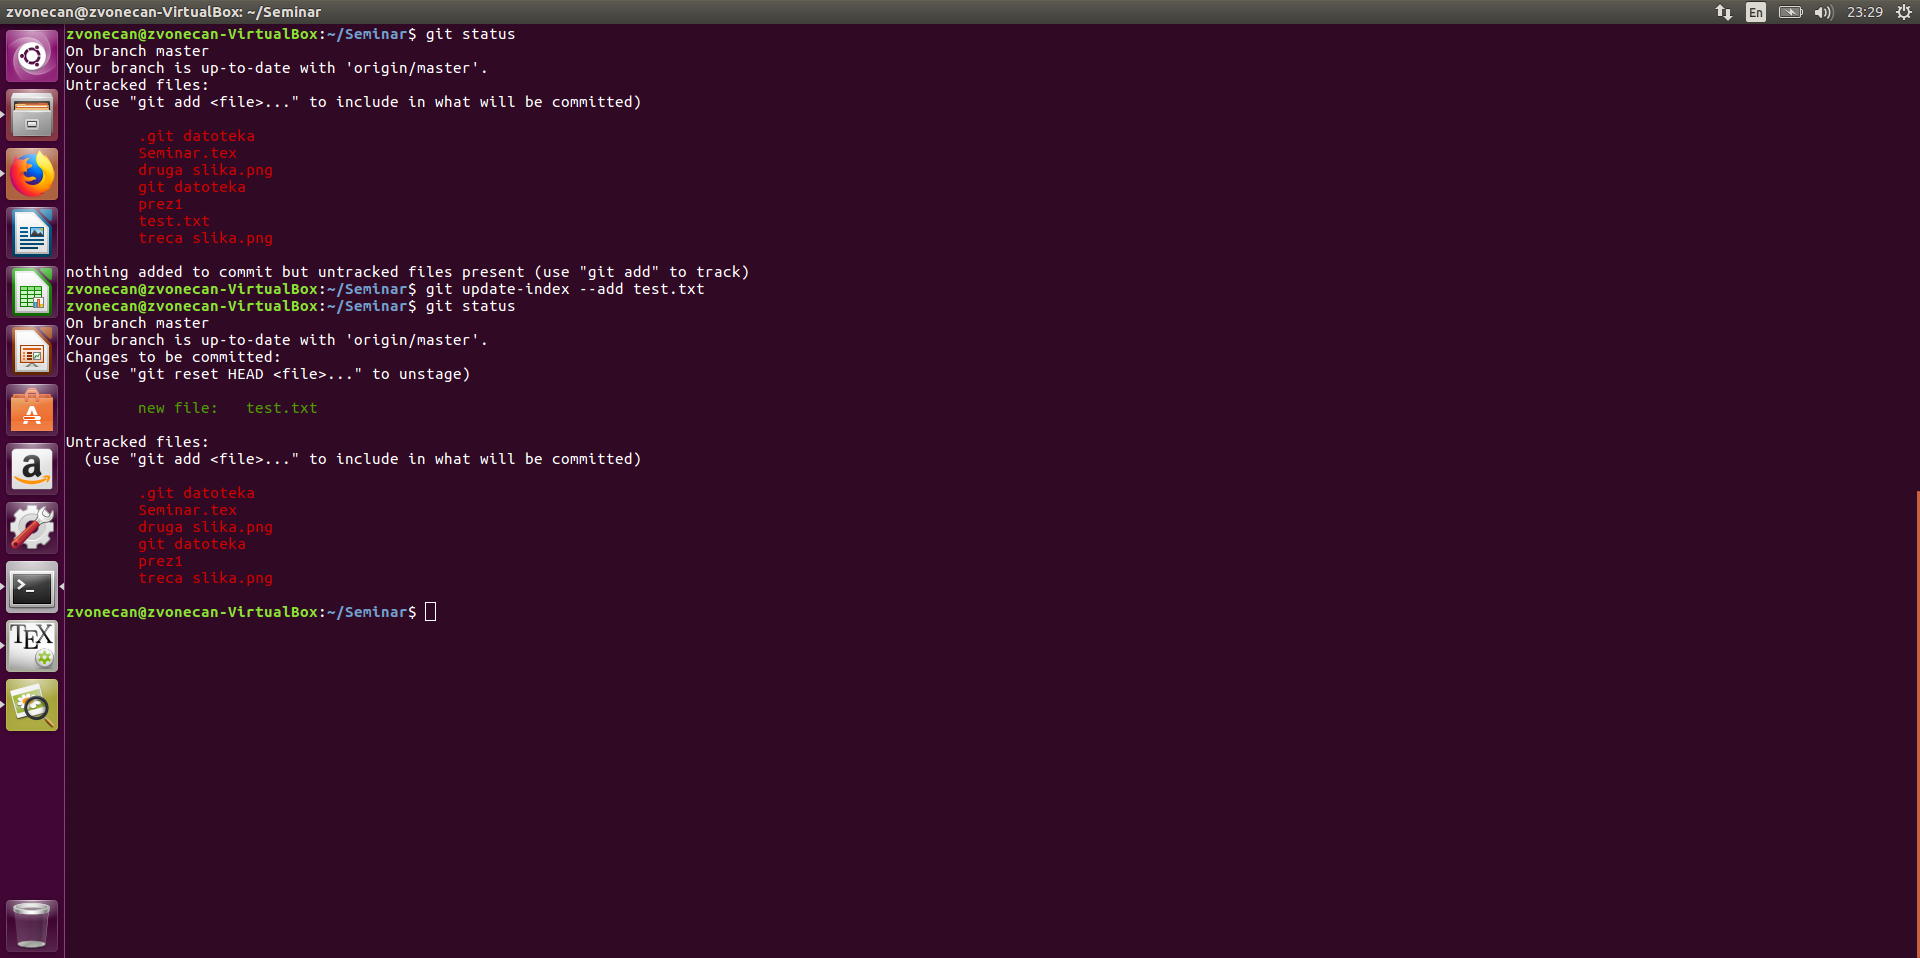
\includegraphics[width=0.7\textwidth]{./slike/cetvrta_slika.png}
	\end{figure}
	\item Ako želimo stagea neki prijašnji commit prije imena filea moramo dodat --cached i SHA-1 tog filea.
	\item Sad mozemo napraviti istu stvar što git radi sa fileovima u indexu , stablo.
	
		
\end{itemize}


\end{frame}
\begin{frame}{git stage}
	\begin{figure}
		\centering
	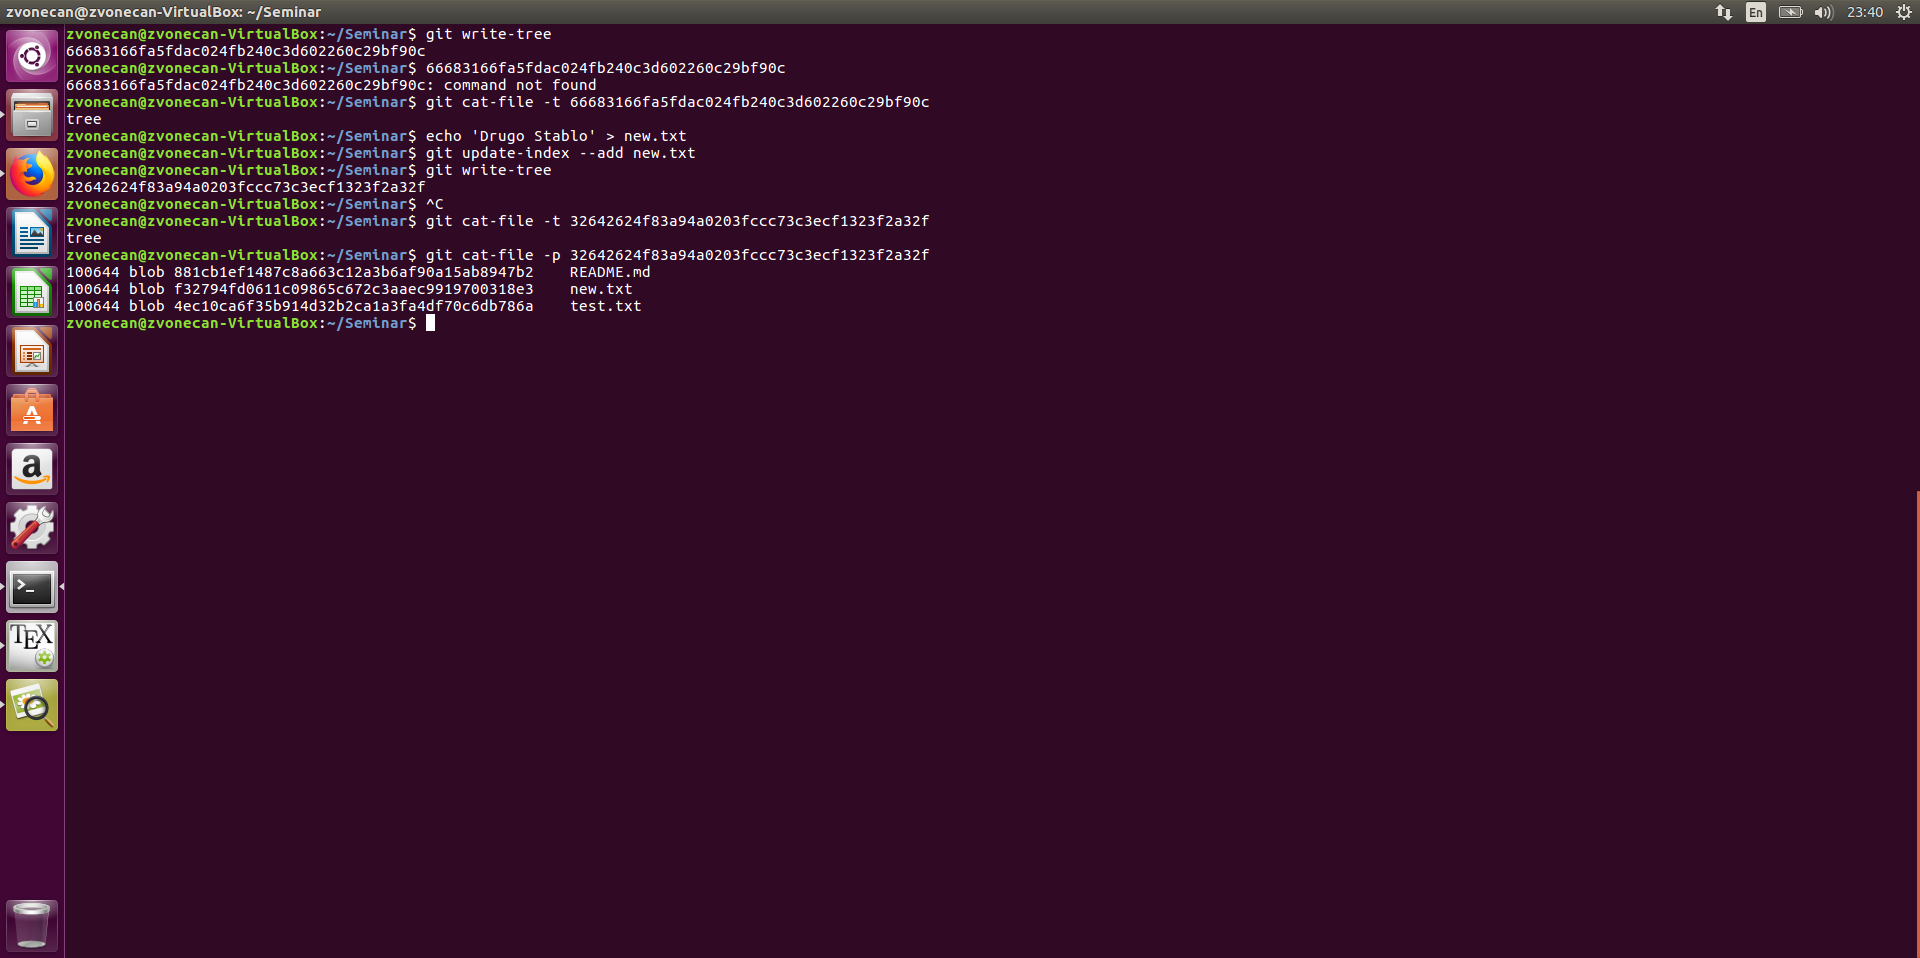
\includegraphics[width=0.7\textwidth]{./slike/peta_slika.png}
	\end{figure}
\end{frame}

\begin{frame}{git stage}
	\begin{figure}
		\centering
	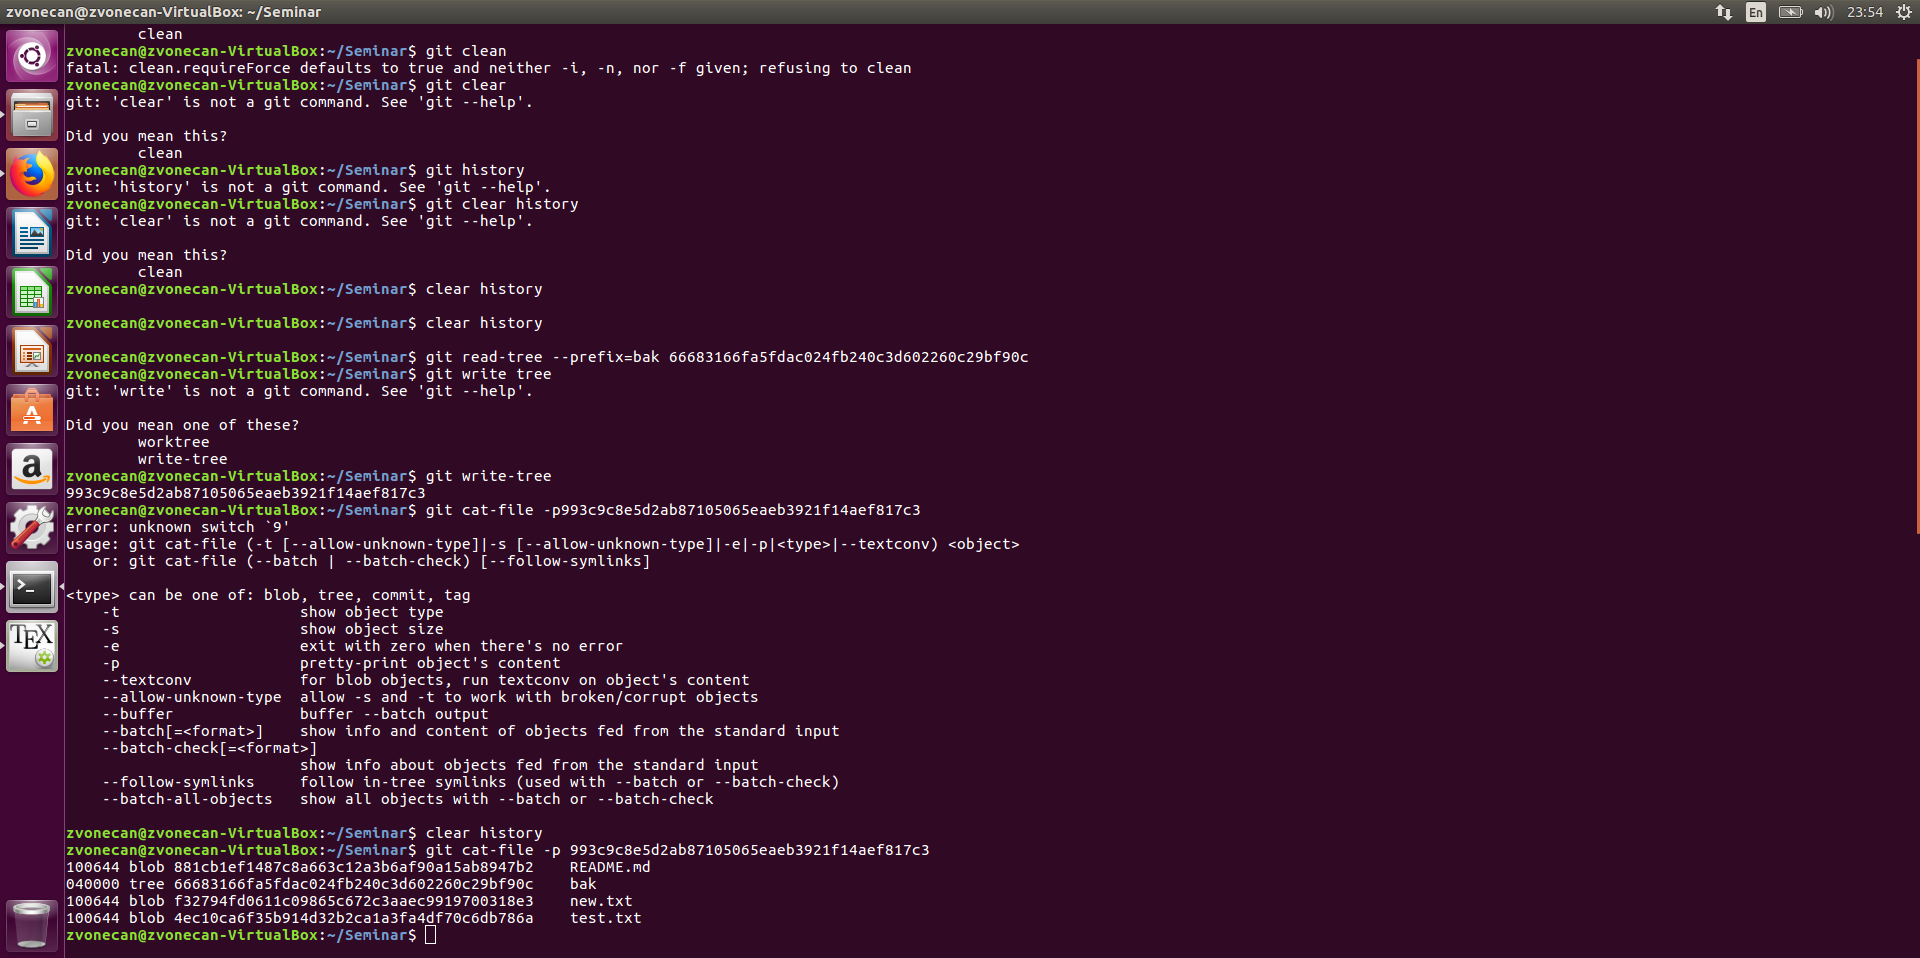
\includegraphics[width=0.8\textwidth]{./slike/sesta_slika.png}
	\end{figure}


\end{frame}

\begin{frame}{git commit}

\begin{itemize}
	\item Sad samo commitamo stablo koje smo napravili te smo izvršili istu stvar koju git napravi kada nešto addamo i commitamo.
	\begin{figure}
		\centering
	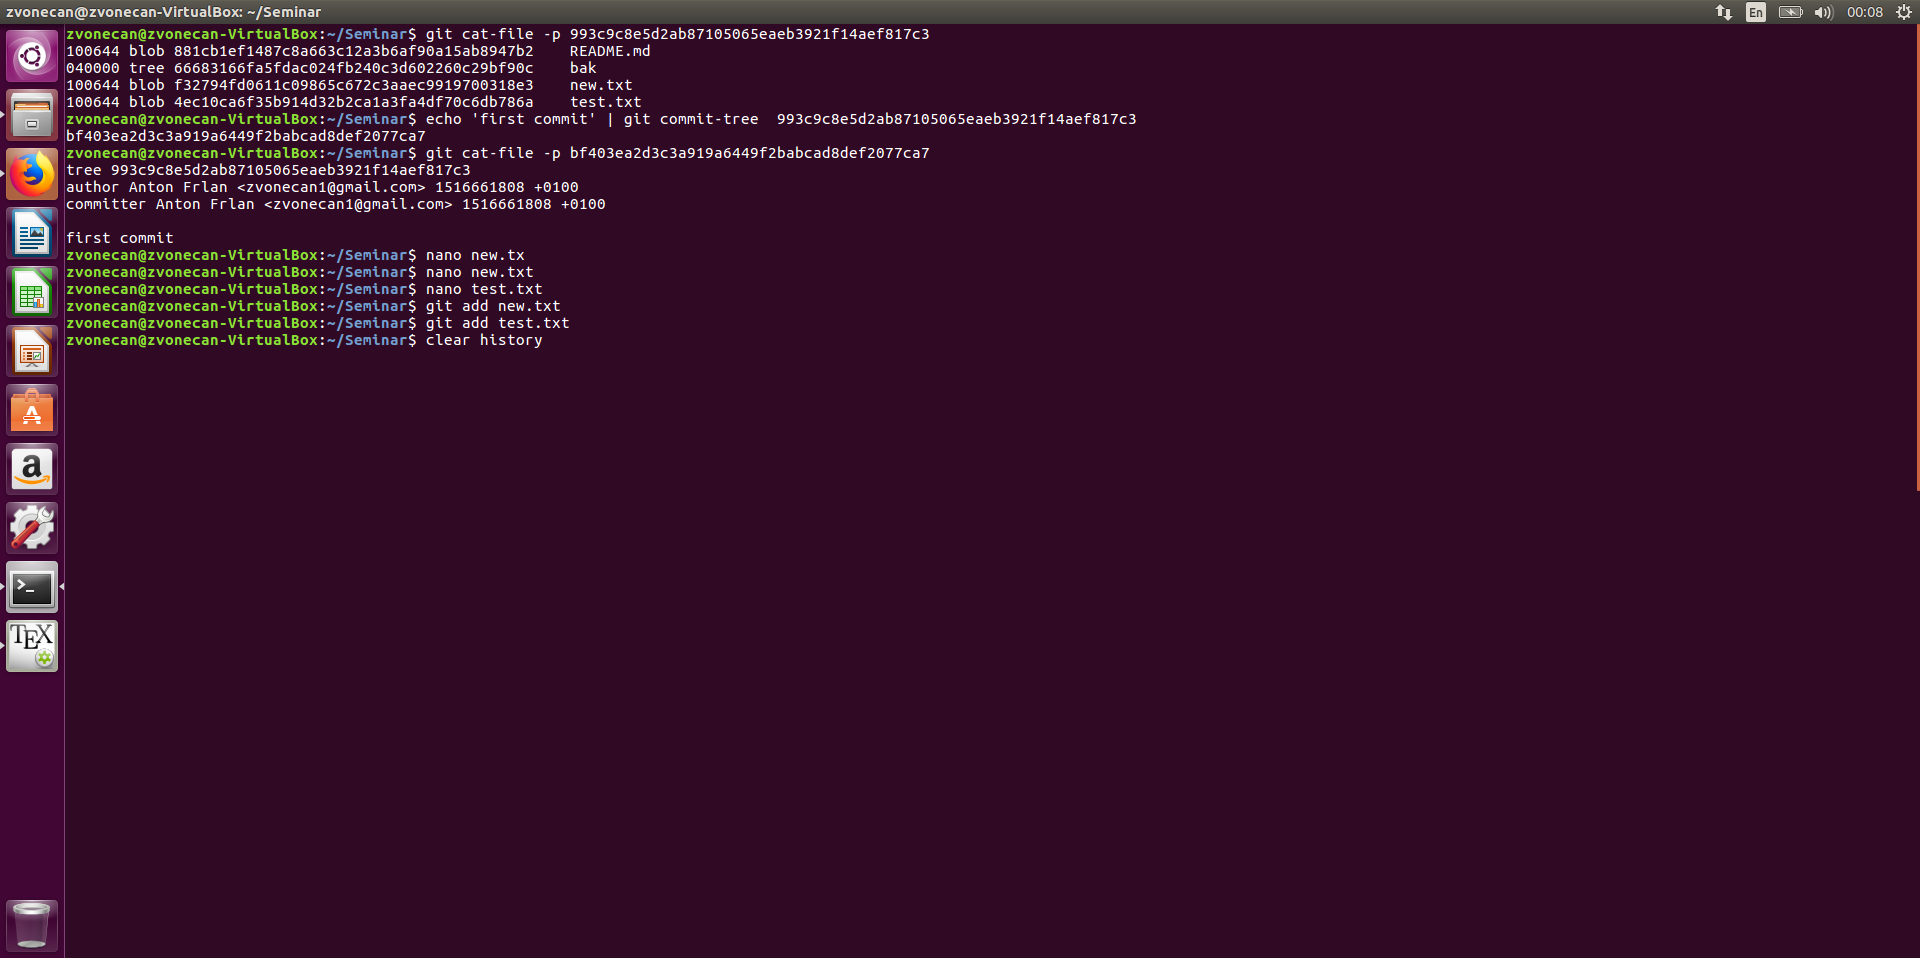
\includegraphics[width=.8\textwidth]{./slike/sedma_slika.png}
	\end{figure}
\end{itemize}
\end{frame}
\begin{frame}{Branching}
	\begin{itemize}
	\item Jedna on najbitnijih stvari u gitu je grananje.
	\item Ono omogućuje razvijanje i debugiranje zasebnih featura bez remećenja glavnog programa. 
	\item Za ovo se mogu koristi reference koje zamijene neki SHA-1 proizvoljnim imenom i odonda se toj novoj grani moze pristupati tim imenom, to jest prati HEAD te grane.
	\end{itemize}
	
\end{frame}
\begin{frame}{Branching}
\begin{figure}
		\centering
	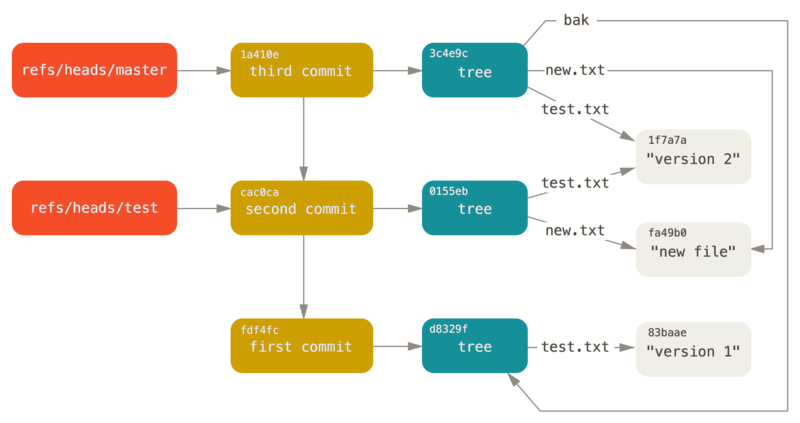
\includegraphics[width=1\textwidth]{./slike/a.png}
	\end{figure}
\end{frame}

\begin{frame}{Merge}
\begin{itemize}
	\item Git merge uspoređuje znakove na svim lokacijama i ako postoje mjesta na kojima nisu isti ih odvoji i stavi jedno ispod drugog.
\end{itemize}
\begin{figure}
		\centering
	
\includegraphics[width=.6\textwidth]{./slike/merge1.png}
	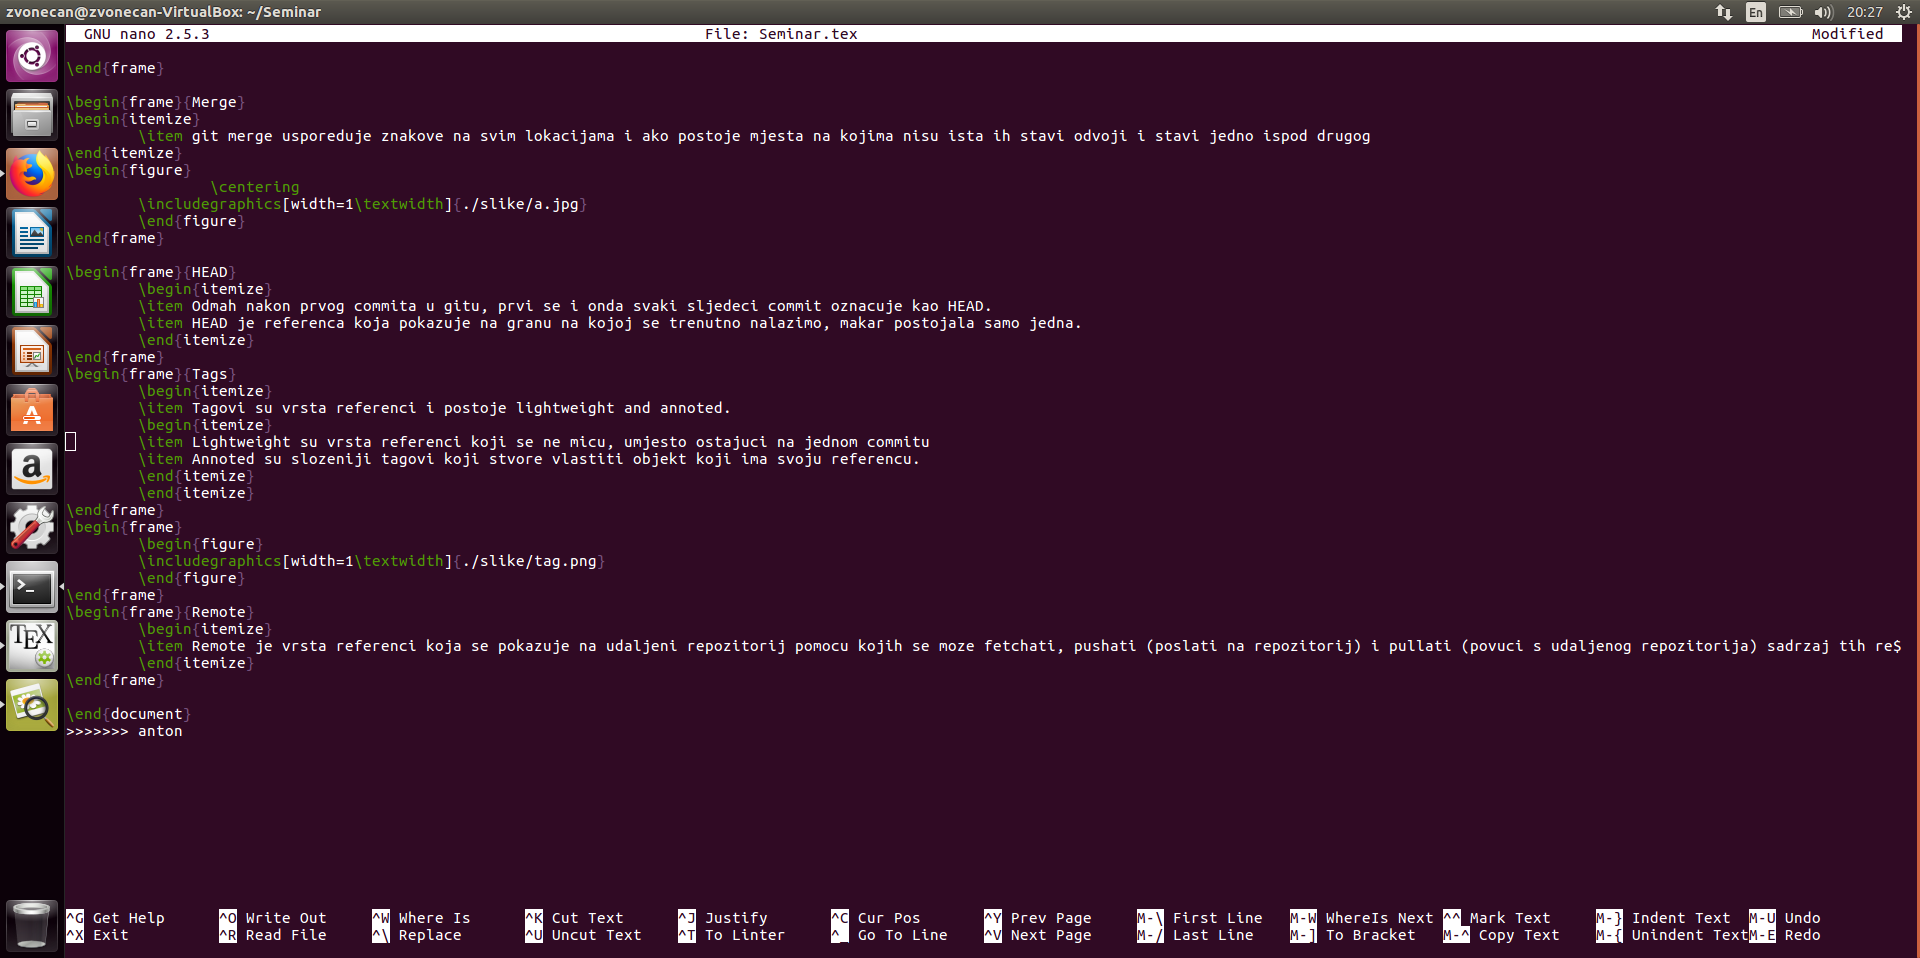
\includegraphics[width=.6\textwidth]{./slike/merge2.png}
	\end{figure}
\end{frame}

\begin{frame}{Merge}
\begin{figure}
		\centering
	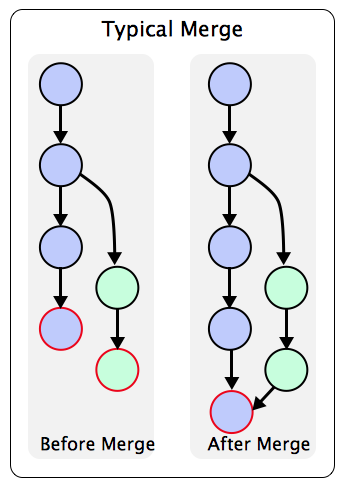
\includegraphics[width=.6\textwidth]{./slike/git_merge.png}
	\end{figure}
\end{frame}

\begin{frame}{HEAD}
	\begin{itemize}
	\item Odmah nakon prvog commita u gitu, prvi se i onda svaki sljedeći commit oznacuje kao HEAD.
	\item HEAD je referenca koja pokazuje na granu na kojoj se trenutno nalazimo, makar postojala samo jedna.
	\end{itemize}
\end{frame}
\begin{frame}{Tags}
	\begin{itemize}
	\item Tagovi su vrsta referenci i postoje lightweight and annoted.
	\begin{itemize}
	\item Lightweight su vrsta referenci koji se ne miču, umjesto ostajući na jednom commitu
	\item Annoted su složeniji tagovi koji stvore vlastiti objekt koji ima svoju referencu.
	\end{itemize}
	\end{itemize}
\end{frame}
\begin{frame}
	\begin{figure}
	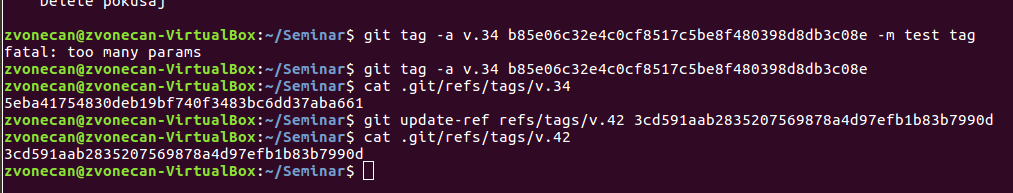
\includegraphics[width=1\textwidth]{./slike/tag.png}
	\end{figure}
\end{frame}
\begin{frame}{Remote}
	\begin{itemize}
	\item Remote je vrsta referenci koja se pokazuje na udaljeni repozitorij pomoću kojih se može fetchati(povući s udaljenog repozitorija da mozemo pogledati sadržaj), pushati (poslati na repozitorij) i pullati (povucć s udaljenog repozitorija te mergati) sadržaj tih repozitorija.  
	\end{itemize}
\end{frame}

\begin{frame}{Remov, diff i status}
	\begin{itemize}
	\item Remove služi za brisanje pojedinih fileova iz trenutačne datoteke.
	\item Status uspoređuje zadnju commitanu verziju s onim sto je napisano poslije i gleda jesu li te razlike stageane kako bi se mogle commitati.
	\item Diff uspoređuje razlike izmedu zadnje commitane verzije i prvo stageanih promjena, ako nema onda svih promjena te ih ispisuje, a dodatci su zeleni i označeni s plusom, a što je izbrisano je crveno s minusom.
	\end{itemize}
\end{frame}
\begin{frame}
\begin{figure}
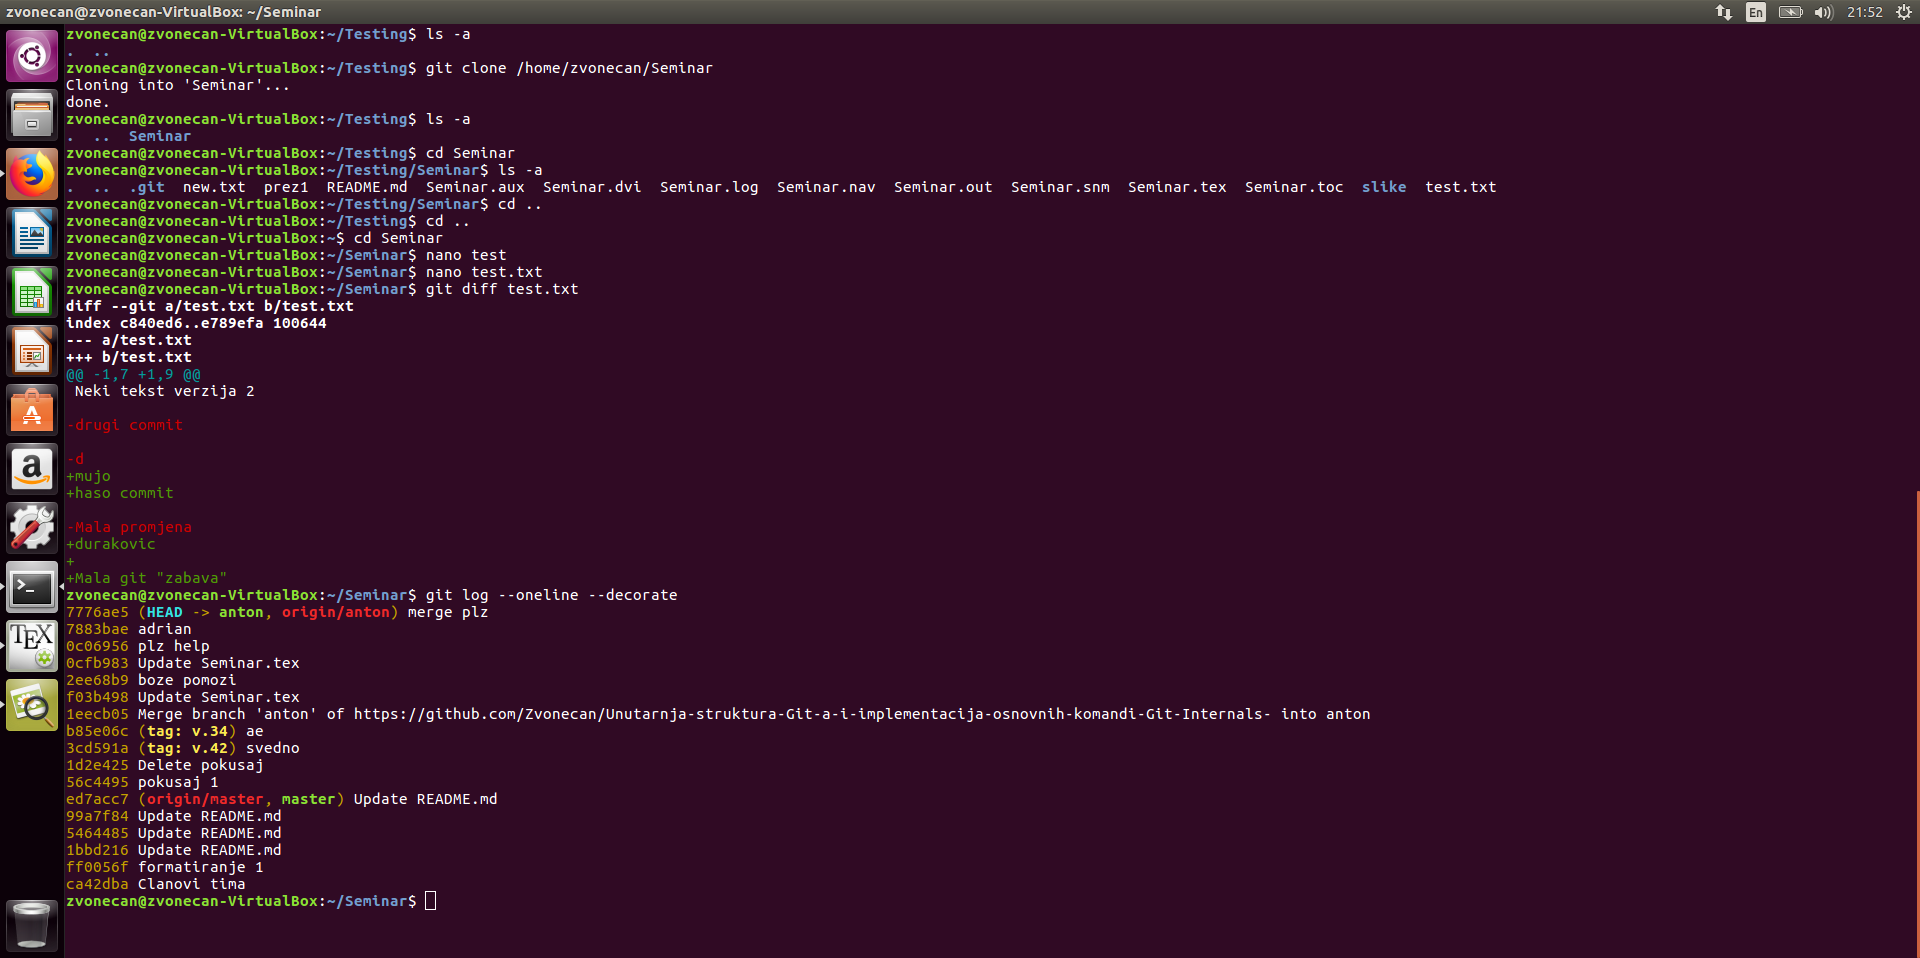
\includegraphics[width=1\textwidth]{./slike/c.png}
\end{figure}
\end{frame}
\begin{frame}{Log i stash}
	\begin{itemize}
	\item Log pokazuje povijest pojedinih grana. Tu se broje commitovi, autor, datum, vrijeme i reference.
	\item Stash privremeno sakriva necommitane promjene ako se iz nekih razloga treba nešto napraviti bez njih. Promjene ostaju skrivene u stashu dok ih se ne povrati nazad na stage.
\end{frame}


\end{document}
